
\section{La Distribución Binomial}


 Si $p$ es la probabilidad de que en un solo ensayo ocurra un evento (llamada la probabilidad de éxito) y $q = 1 - p$ es la
probabilidad de que este evento no ocurra en un solo ensayo (llamada probabilidad de fracaso), entonces la probabilidad de que el evento ocurra exactamente $x$ veces en $N$ ensayos (es decir, que ocurran $x$ éxitos y $N - x$ fracasos) está
dada por
\begin{align}
 \label{eq:7.1}
 f(x)=P(X=x)=\comb{N}{x}p^{x}q^{N-x}
\end{align}
donde $x=0,1,...,N.$


 \begin{exmp}
  \label{exmp:7.1}
  La probabilidad de obtener exactamente dos caras en seis lanzamientos de una moneda es
  \begin{align*}
   \comb{6}{2}\left( \dfrac{1}{2} \right)^{2}\left( \dfrac{1}{2} \right)^{6-2}=\dfrac{15}{64}
  \end{align*}
empleando \eqref{eq:7.1} con $N=6, x=2, p=q=\frac{1}{2}.$
 \end{exmp}



\begin{exmp}
 \label{exmp:7.2}
 Calcule la probabilidad de obtener al menos 4 caras en 6 lanzamientos de una moneda.
\end{exmp}



 En lo subsecuente, daremos por hecho que hemos importado los siguientes paquetes:
 \begin{itemize}
  \item \texttt{scipy.stats}
  \item \texttt{numpy} como \texttt{np}
 \end{itemize}


[fragile, allowframebreaks]{statsBinom.py}
\begin{verbatim}
from scipy import stats
import numpy as np
import matplotlib.pyplot as plt

#Consideremos 6 experimentos con p de éxito 1/2
p=0.5
N=6
binDist = stats.binom(N,p)
#probabilidad de obtener dos éxitos
print binDist.pmf(2)
##0.234375
#probabilidad de obtener al menos 4 éxitos
print sum(binDist.pmf(np.arange(4,6+1)))
##0.34375
 \end{verbatim}


 \begin{exmp}
  \label{exmp:7.3}
  Desarrolle $\left( p+q \right)^{4}.$
 \end{exmp}


[fragile, allowframebreaks]{coefBinom.py}
\begin{verbatim}

from scipy import stats
import numpy as np

#coeficientes de (p+q)^4
p=.5
N=4
binomDist = stats.binom(N,p)
binDistExmp = binomDist.pmf(np.arange(5))
print binDistExmp*2**N
##[ 1.  4.  6.  4.  1.]
\end{verbatim}


{Propiedades de la distribución binomial} Supongamos que realizamos $N$ experimentos con probabilidad éxito $p$ y de fracaso $q=1-p.$
\begin{align}
 \label{binom:mean}
 \mu = Np \\
 \label{binom:var}
 \s^{2}=Npq
\end{align}


[fragile,allowframebreaks]{histBinom.py}
 \begin{verbatim}
import numpy as np
import matplotlib.pyplot as plt

#Ejemplo de distribución binomial
N,p=100, 0.5
s = np.random.binomial(N,p,1000)

miHist = np.histogram(s, bins = np.arange(100+1))
print miHist[0]
print miHist[1]
print np.mean(s)
print N*p
print np.var(s)
print N*p*(1-p)

plt.hist(s, bins = np.arange(100+1))
plt.show()
 \end{verbatim}




 \begin{figure}[h]
 \centering
 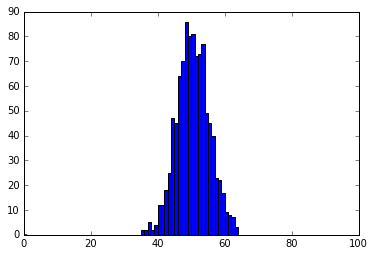
\includegraphics[height=7cm,keepaspectratio=true]{./pe/distBin01.png}
 % distBin01.png: 0x0 pixel, 300dpi, 0.00x0.00 cm, bb=
 \label{distBin01}
\end{figure}


\section{Distribución Normal}

 Una de las distribuciones de probabilidad continua más importantes es la \emph{distribución normal}, también llamada \emph{distribución gaussiana,} que se define mediante la función de densidad
 \begin{align}
  \label{eq:7.3_}
  f_{a,b}(x)=\dfrac{1}{\sqrt{2\pi}}e^{-\frac{1}{2}\frac{(x-a)^{2}}{b^{2}}}
 \end{align}
donde $a,b$ son parámetros específicos para cada v.a. $X.$

{Propiedades de la distribución normal}
 Si la v.a. $X$ tiene la función de densidad dada por \eqref{eq:7.3_}, con parámetros $a,b$ entonces
 \begin{align}
  a = \mu_{X}\\
  b = \s_{X}
 \end{align}



 Si una variable aleatoria normal $X$ tiene función de densidad
  \begin{align}
  \label{eq:7.3_}
  f(x)=\dfrac{1}{\sqrt{2\pi}}e^{-\frac{1}{2}\frac{(x-\mu)^{2}}{\s^{2}}},
 \end{align}
 escribiremos $X\sim N(\mu, \s^{2}).$


{Variable aleatoria normalizada}
 \begin{align}
  \label{van}
  Z = \dfrac{X-\mu}{\s}\\
  \mu_{Z}=0 \\
  \s_{Z}=1
 \end{align}


{Forma Estándar}
 \begin{align}
  \label{eq:7.4}
  f(z)=\dfrac{1}{\sqrt{2\pi}}e^{-\frac{1}{2}z^{2}}
 \end{align}


En este caso, diremos que $Z$ está \emph{normalmente distribuida.}


[fragile, allowframebreaks]{distribucionNormal.py}
 \begin{verbatim}
import scipy.integrate as integrate
import numpy as np
import matplotlib.pyplot as plt
from matplotlib.patches import Polygon

def fn(x,m=0,s=1):
    return np.exp(-(x-m)**2/(2*s**2))/(s*np.sqrt(2*np.pi))
x1 = np.arange(-4,4,0.1)
plt.plot(x1, fn(x1))
plt.show()

for s in np.arange(1,4+1):
    result = integrate.quad(lambda x:fn(x),-s,s)
    print result

for s in np.arange(1,4+1):
    result = integrate.quad(lambda x:fn(x),-s,s)

    a, b = -s, s  # integral limits
    x = np.arange(-4,4,0.01)
    y = fn(x)

    fig, ax = plt.subplots()
    plt.plot(x, y, 'r', linewidth=2)
    plt.ylim(ymin=0)

    # Make the shaded region
    ix = np.linspace(a, b)
    iy = fn(ix)
    verts = [(a, 0)] + list(zip(ix, iy)) + [(b, 0)]
    poly = Polygon(verts, facecolor='0.9', edgecolor='0.5')
    ax.add_patch(poly)

    ax.set_xticks((a, b))
    ax.set_xticklabels(('$-\sigma$', '$\sigma$'))
    ax.set_yticks([])

    plt.show()
    print result
 \end{verbatim}


[fragile]
 \begin{figure}[h]
 \centering
 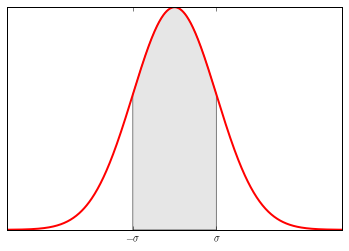
\includegraphics[height=5cm,keepaspectratio=true]{./pe/norm1.png}
 % norm1.png: 0x0 pixel, 300dpi, 0.00x0.00 cm, bb=
 \label{fig:norm1}
\end{figure}
\begin{verbatim}
 #(0.682689492137086, 7.579375928402476e-15)
\end{verbatim}


[fragile]
 \begin{figure}[h]
 \centering
 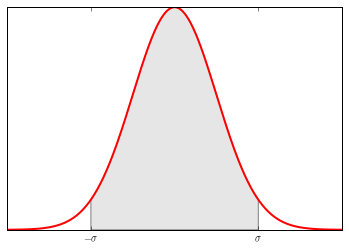
\includegraphics[height=5cm,keepaspectratio=true]{./pe/norm2.png}
 % norm1.png: 0x0 pixel, 300dpi, 0.00x0.00 cm, bb=
 \label{fig:norm2}
\end{figure}
\begin{verbatim}
 #(0.9544997361036417, 1.8403548653972355e-11)
\end{verbatim}


[fragile]
 \begin{figure}[h]
 \centering
 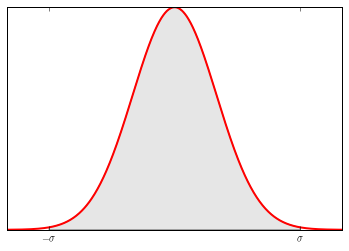
\includegraphics[height=5cm,keepaspectratio=true]{./pe/norm3.png}
 % norm1.png: 0x0 pixel, 300dpi, 0.00x0.00 cm, bb=
 \label{fig:norm3}
\end{figure}
\begin{verbatim}
 #(0.9973002039367399, 1.1072256503105314e-14)
\end{verbatim}


[fragile]
 \begin{figure}[h]
 \centering
 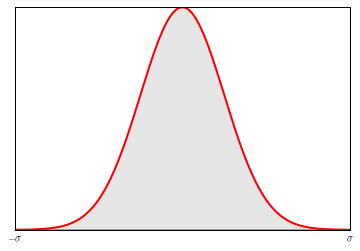
\includegraphics[height=5cm,keepaspectratio=true]{./pe/norm4.png}
 % norm1.png: 0x0 pixel, 300dpi, 0.00x0.00 cm, bb=
 \label{fig:norm4}
\end{figure}
\begin{verbatim}
 #(0.9999366575163339, 4.838904125482879e-12)
\end{verbatim}


[fragile, allowframebreaks]{normalCDF.py}
 \begin{verbatim}
from scipy import stats
import numpy as np
import matplotlib.pyplot as plt

mu = 3.5
sigma = 0.76
nd = stats.norm(mu, sigma)

x = np.arange(mu - 4*sigma,mu + 4*sigma,0.01)
y = nd.cdf(x)

fig, ax = plt.subplots()
plt.plot(x, y, 'r', linewidth=2)
plt.ylim(ymin=0)

for k in range(1,5):
    print nd.cdf(mu+k*sigma)-nd.cdf(mu-k*sigma)

#0.682689492137
#0.954499736104
#0.997300203937
#0.999936657516
 \end{verbatim}
\begin{center}
 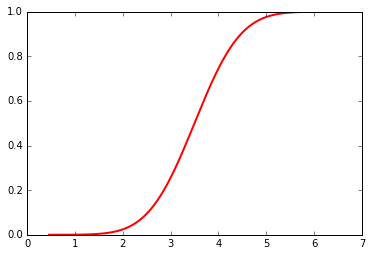
\includegraphics[height=5cm,keepaspectratio=true]{./pe/normCDF.png}
 % normCDF.png: 0x0 pixel, 300dpi, 0.00x0.00 cm, bb=
\end{center}



\section{Relación entre las distribuciones binomial y normal}

 Si $N\sim \infty, p,q>>0,$ y $X$ es un distribución binomial con parámetros $N,p$ entonces
 \begin{align}
  \dfrac{X-Np}{\sqrt{Npq}} \sim N(0,1).
 \end{align}



 \begin{exmp}
  \label{exmp:7.5}
  Consideremos el experimento de lanzar 16 veces una moneda. Repitamos 1,000,000 dicho experimento. Compruebe que dicho experimento se puede modelar por una variable aleatoria con distribución $N(\mu=8,\sigma^{2}=4)$
 \end{exmp}


[fragile, allowframebreaks]{relBinomNormal.py}
 \begin{verbatim}
import numpy as np
import matplotlib.pyplot as plt

def fn(x,m=0,s=1):
    C = 1/(s*np.sqrt(2*np.pi))
    return C*np.exp(-(x-m)**2/(2*s**2))

N,p=30, 0.5
R = 1000000
q=1-p
mB = N*p
sB = np.sqrt(N*p*q)
X = np.random.binomial(N,p,R)
myBins = np.arange(-0.5,N+0.5,1)
plt.hist(X, bins = myBins)
x = np.arange(mB-4*sB,mB+4*sB+0.1,0.1)
y = R*fn(x, m=mB, s=sB)
plt.plot(x,y,lw=2)
plt.ylim(ymin=0)
plt.show()
 \end{verbatim}
\begin{center}
 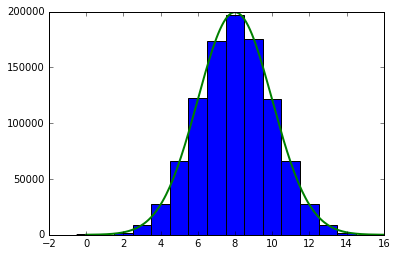
\includegraphics[height=5cm]{./pe/relBinNorm.png}
 % relBinNorm.png: 0x0 pixel, 300dpi, 0.00x0.00 cm, bb=
\end{center}



\section{La Distribución de Poisson}
{Distribución de Poisson} Diremos que una variable aleatoria \emph{discreta} $X$ tiene distribución de Poisson si su función de probabilidad está dada por:
 \begin{align}
  \label{eq:7.5}
  f(n)=\dfrac{\lam^{n}e^{-\lam}}{n!}, \; n=0,1,2,...
 \end{align}


En este caso, $\mu_{X}=\s^{2}=\lam.$


\begin{quote}
 En teoría de probabilidad y estadística, la distribución de Poisson es una distribución de probabilidad discreta que expresa, a partir de una frecuencia de ocurrencia media, la probabilidad de que ocurra un determinado número de eventos durante cierto período de tiempo. Concretamente, se especializa en la probabilidad de ocurrencia de sucesos con probabilidades muy pequeñas, o sucesos raros.
\end{quote}

\href{https://es.wikipedia.org/wiki/Distribuci\%C3\%B3n_de_Poisson}{Wikipedia: Distribución de Poisson}


 \begin{exmp}
  \label{exmp:7.6}
  El número de personas por día que llegan a una sala de urgencias tiene una distribución de Poisson con media 5. Hallar la probabilidad de que cuando mucho lleguen tres por día y la probabilidad de que por lo menos lleguen 8 personas por día.
 \end{exmp}




[fragile, allowframebreaks]{distPoisson.py}
 \begin{verbatim}
from scipy import stats
import numpy as np
import matplotlib.pyplot as plt

def f(x, mu=1):
    return stats.poisson.pmf(x, mu)

def F(x, mu=1):
    return stats.poisson.cdf(x, mu)

x1 = np.arange(0,100+1)
plt.plot(x1, f(x1, mu=5), 'bo')
plt.show()

s = np.random.poisson(5,365)
M = np.max(s)
myBins = np.arange(0,M+1)
plt.hist(s, bins = myBins)
plt.show()

print F(3, mu=5)
print 1 - F(7, mu=5)

for k in range(12+1):
    print k, F(k, 5)
"""
0 0.00673794699909
1 0.0404276819945
2 0.124652019483
3 0.265025915297
4 0.440493285065
5 0.615960654833
6 0.762183462973
7 0.86662832593
8 0.931906365278
9 0.968171942694
10 0.986304731402
11 0.994546908087
12 0.997981148373
"""
 \end{verbatim}



 \begin{figure}[h]
 \centering
 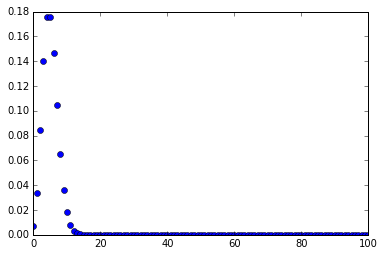
\includegraphics[height=7cm,keepaspectratio=true]{./pe/distPoisson0.png}
 % distPoisson0.png: 0x0 pixel, 300dpi, 0.00x0.00 cm, bb=
 \caption{Distribución de Poisson}
\end{figure}




\begin{figure}[h]
 \centering
 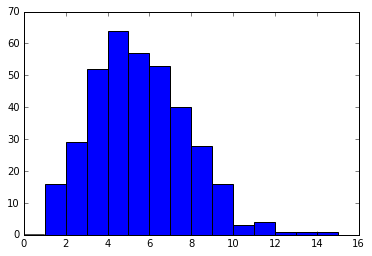
\includegraphics[height=7cm,keepaspectratio=true]{./pe/distPoisson1.png}
 % distPoisson1.png: 0x0 pixel, 300dpi, 0.00x0.00 cm, bb=
 \caption{Histograma de pacientes en sala de urgencias durante un año con media $\lam=5$}
 \label{fig:distPoisson1}
\end{figure}



\section{Relación entre las Distribuciones Binomiales y de Poisson}

 Si en la función de probabilidad binomial, $N$ es muy grande pero $p \approx 0,$ esto modela un \emph{evento raro}.  En la práctica esto significa $N>>50, Np<<5.$ 

 En este caso, la distribución Binomial con parámetros $N,p$ se aproxima a una Poisson con parámetro $\lam = Np.$

[fragile, allowframebreaks]{relBinomPoisson.py}
 \begin{verbatim}
from scipy import stats
import numpy as np
import matplotlib.pyplot as plt
import matplotlib as mpl

mpl.style.use("ggplot")

fig, ax = plt.subplots(1, 1)

def fP(x, mu=1):
    return stats.poisson.pmf(x, mu)

def fB(x, N=30, p=0.5):
    return stats.binom(N,p).pmf(x)

N_=50
p_=5./N_
mu_ = N_*p_
x1 = np.arange(0,20+1)
ax.plot(x1, fP(x1, mu=mu_), 'bo', label="Poisson")
ax.plot(x1, fB(x1, N=N_, p=p_), 'ro', label="Binomial")
legend = ax.legend(loc='upper center', shadow=True)
plt.show()

 \end{verbatim}



 \begin{figure}[h]
 \centering
 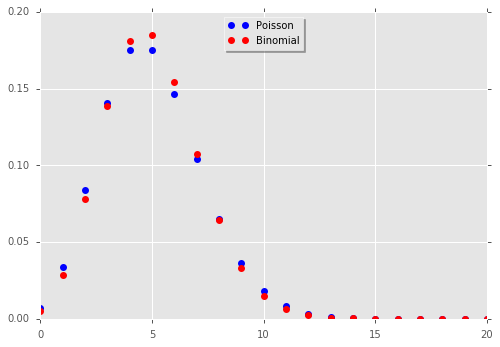
\includegraphics[height=7cm]{./pe/binVsPoi.png}
 % binVsPoi.png: 0x0 pixel, 300dpi, 0.00x0.00 cm, bb=
 \caption{Comparación entre distribuciones Binomial y Poisson para eventos raros.}
\end{figure}



\section{Distribución multinomial}

 Si los eventos $E_{1},...,E_{k}$ pueden ocurrir con probabilidades $p_{1},...,p_{k}$ respectivamente, entonces la probabilidad de que ocurran $X_{1},...,x_{k}$ veces respectivamente esta dado por la \emph{distribución multinomial}
 \begin{align}
  \label{eq:7.6}
  f\left( x_{1},...,x_{2} \right)=
  \dfrac{x_{1}+...+x_{k}}{x_{1}!...x_{k}!}p_{1}^{x_{1}}\cdots p_{k}^{x_{k}}.
 \end{align}



 \begin{exmp}
  \label{exmp:7.7}
Si un dado se lanza 12 veces, encontrar la probabilidad de obtener cada uno de los números $1,2,3,4,5,6$ exactamente dos veces.
 \end{exmp}



\section{Problemas Resueltos}
{Percentil}
 Diremos que $x=P_{q}$ es el percentil $q, \; 0\leq q \leq 100$ de la distribución $F(x)$ si $F(P_{q})=q\%.$  En el caso de que $q$ sea un valor realizable de $F(x),$ podemos \emph{``despejar''}
 \begin{align}
  P_{q}=F^{-1}\left( \dfrac{q}{100} \right).
 \end{align}
 A tal función se le llama \emph{distribución inversa.}


{Cuartiles}
 En la literatura se definen conceptos similares. Por ejemplo, el primer \emph{cuartil} corresponde al percentil $25;$ el segundo cuartil al percentil $50;$ y así sucesivamente.

{Combinaciones}
 \begin{exmp}
  \label{sol:7.1}
  Encuentre
  \begin{enumerate}[(a)]
   \item $5!$
   \item $\comb{8}{3}$
  \end{enumerate}
  utilizando \texttt{Python.}
 \end{exmp}


[fragile, allowframebreaks]{combinaciones.py}
 \begin{verbatim}
import math
import scipy.special

print math.factorial(5)
print scipy.special.binom(8,3)
 \end{verbatim}




{Distribución Binomial}
 \begin{exmp}
  \label{sol:7.2}
  Supóngase que $15\%$ de la población es zurda. Encontrar la probabilidad de que en un grupo de 50 individuos haya:
  \begin{enumerate}[(a)]
   \item cuando mucho 10 zurdos; 
   \item por lo menos 5 zurdos; 
   \item entre 3 y 6 zurdos; 
   \item exactamente 5 zurdos.
  \end{enumerate}

 \end{exmp}


[fragile, allowframebreaks]{solvedBinom.py}
 \begin{verbatim}
from scipy import stats

#7.2 N=50, p=15%
def f(x):
    return stats.binom(50,.15).pmf(x)
def F(x):
    return stats.binom(50,.15).cdf(x)
#(a) P(X<=10)
print sum([f(x) for x in range(0,10+1)])
##0.8800826828
print F(10)
##0.8800826828
#(b) P(X>=5)
print 1-sum([f(x) for x in range(0,4+1)])
##0.887894791945
print 1-F(4)
##0.887894791945
#(c) P(3<=X<=6)
print sum([f(x) for x in range(3,6+1)])
##0.3471108697
print F(6)-F(2)
##0.3471108697
#(d) P(X=5)
print f(5)
##0.3471108697
 \end{verbatim}



{Distribución Normal}
 \begin{exmp}
  \label{sol:7.14}
  En un examen final de matemáticas, la media fue 72 y la desviación estándar fue 15. Determinar las puntuaciones estándar de los estudiantes que obtuvieron:
  \begin{enumerate}[(a)]
   \item $60$;
   \item $93$;
   \item $72$.
  \end{enumerate}

 \end{exmp}



 \begin{exmp}
  \label{sol:7.15}
  Con los datos del problema \ref{sol:7.14}, encontrar las calificaciones que corresponden a las siguientes puntuaciones estándar:
  \begin{enumerate}[(a)]
   \item $-1$;
   \item $1.6$.
  \end{enumerate}

 \end{exmp}



 \begin{exmp}
  \label{sol:7.16}
  Supóngase que la cantidad de juegos en que participan los beisbolistas de la liga mayor durante su carrera se distribuye normalmente con media de $1500$ juegos y desviación estándar $350$ juegos. Emplear \texttt{Python} para responder las siguientes preguntas:
  \begin{enumerate}[(a)]
   \item ¿Qué porcentaje participa en menos de 750 juegos?;
   \item ¿qué porcentaje participa en más de 2000 juegos?;
   \item encontrar el \emph{percentil} $90$ de la cantidad de juegos en los que participan en su carrera.
  \end{enumerate}

 \end{exmp}


[fragile, allowframebreaks]{solvedNorm.py}
 \begin{verbatim}
from scipy import stats

mu = 1500
sigma = 350
nd = stats.norm(mu, sigma)

def F(x):
    return nd.cdf(x)

#a
print F(750)
##0.3471108697

#b
print 1-F(2000)
##0.0765637255098

def inverseF(x):
    return nd.ppf(x)
#c
print inverseF(.90)
##1948.54304794
 \end{verbatim}


{Eventos raros}
\begin{exmp}
\label{sol:7.28}
  Si la probabilidad de que un individuo tenga una reacción adversa por la inyección de determinado suero es $0.001,$ determinar la probabilidad de que de 2000 individuos:
 \begin{enumerate}[(a)]
  \item exactamente 3;
  \item más de 2
 \end{enumerate}
sufran una reacción adversa.
\end{exmp}


[fragile, allowframebreaks]{eventosRaros.py}
 \begin{verbatim}
from scipy import stats
#7.28
#a
N = 2000
p = 0.001
print stats.binom(N,p).pmf(3)
##0.180537328032
print stats.poisson(N*p).pmf(3)
##0.180447044315
#(b)
print 1-stats.binom(N,p).cdf(2)
##0.32332356124
print 1-stats.poisson(N*p).cdf(2)
##0.323323583817
 \end{verbatim}



\end{document}
